\documentclass{standalone}
\usepackage[dvipsnames]{xcolor}
\usepackage{tikz}
\usepackage{amsmath,amssymb}
\usepackage{bm}
\usetikzlibrary{arrows,intersections,shapes,calc,positioning}

\tikzset{%
insert arc/.style args={#1:#2:#3and#4 with center #5}{
  insert path={
    \pgfextra{%
      \pgfpointxy{#3}{#4}%
      \pgfgetlastxy\arcrx\arcry%
      \pgfcoordinate{#5}{%
        \pgfpoint{\csname tikz@lastx\endcsname+\arcrx*cos(#1+180)}%
          {\csname tikz@lasty\endcsname+\arcry*sin(#1+180)}}
      }
    arc (#1:#2:#3 and #4) 
    }
  }
}

\begin{document}
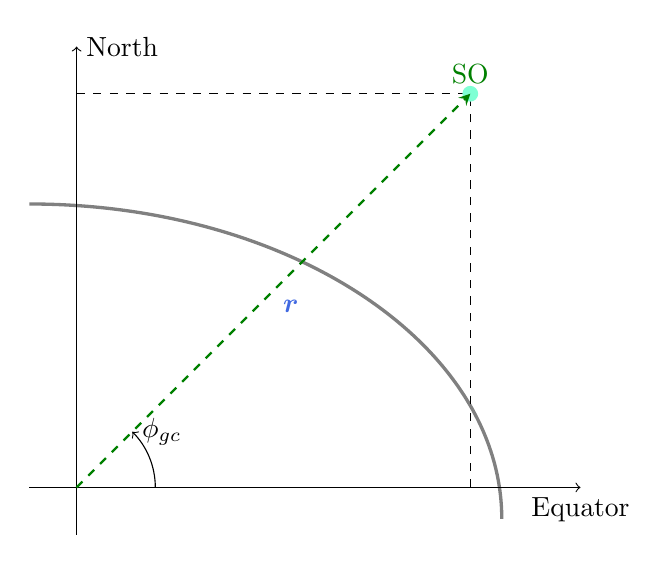
\begin{tikzpicture}[scale = 2,rotate=0]
\draw [very thick, Gray] (2.7,-0.2)  [insert arc={0:90:3 and 2 with center X}];

\draw[->,thin] (-0.3,0) -- (3.2,0) coordinate[label = {below:Equator}] (xmax);
\draw[->] (0,-0.3) -- (0,2.8) coordinate[label = {right:North}] (ymax);

\draw[dashed,thin] (2.5,0) -- (2.5,2.5) coordinate[label= ](Xsatellite);
\draw[dashed,thin] (0,2.5) -- (2.5,2.5) coordinate[label = ];

\begin{scope}
%\filldraw(Xsatellite) circle (0.05);
\path[fill=Aquamarine](Xsatellite)circle(0.05);
\end{scope}

\draw[dashed,Green,thick, -stealth] (0,0) -- (Xsatellite) coordinate[label=SO];
\draw[RoyalBlue] (0.5*2.5,0.5*2.5) node[anchor=north west]{$\bm{r}$};
%\draw (0.1,0.2 ) node[anchor=north west] {$\phi_{gd}$};
\draw[->] (0.5,0) arc (0:45:0.5) node[anchor=west] {$\phi_{gc}$};

%\draw[thick, olive, ->](0,0) -- ({0.99*\r*cos(\t)}, {0.99*\r*sin(\t)});
%\draw [dashed, red] (X) ellipse [x radius=3, y radius=2];

\end{tikzpicture}
\end{document}